\chapter{Robótica evolutiva}
\label{evolutiva}

\section{Introdução}

introdução

\section{Redes Neurais Artificiais (RNA)}

Redes neurais artificias são sistemas computacionais inspirados em sistemas
nervosos animais capazes de aprendizado. Matematicamente, RNAs são aproximadores
universais \cite{hornik89universal}. Um RNA é composto por uma rede de unidades
de processamento simples (neurônios). Cada neurônio possui um sinal de saída e
pode receber um ou mais sinais de entrada.

\subsection{Multi-Layer Perceptron (MLP)}

Uma rede neural MLP é composta por uma série de neurônios organizados em camadas, onde cada neurônio recebe, como entrada, a saída dos neurônios da camada anterior. Uma rede com uma camada intermediária é capaz de aproximar qualquer função contínua. Com duas camadas intermediárias, qualquer função pode ser aproximada \cite{cybenko89mlp}.

\begin{figure}[h]
    \centering
    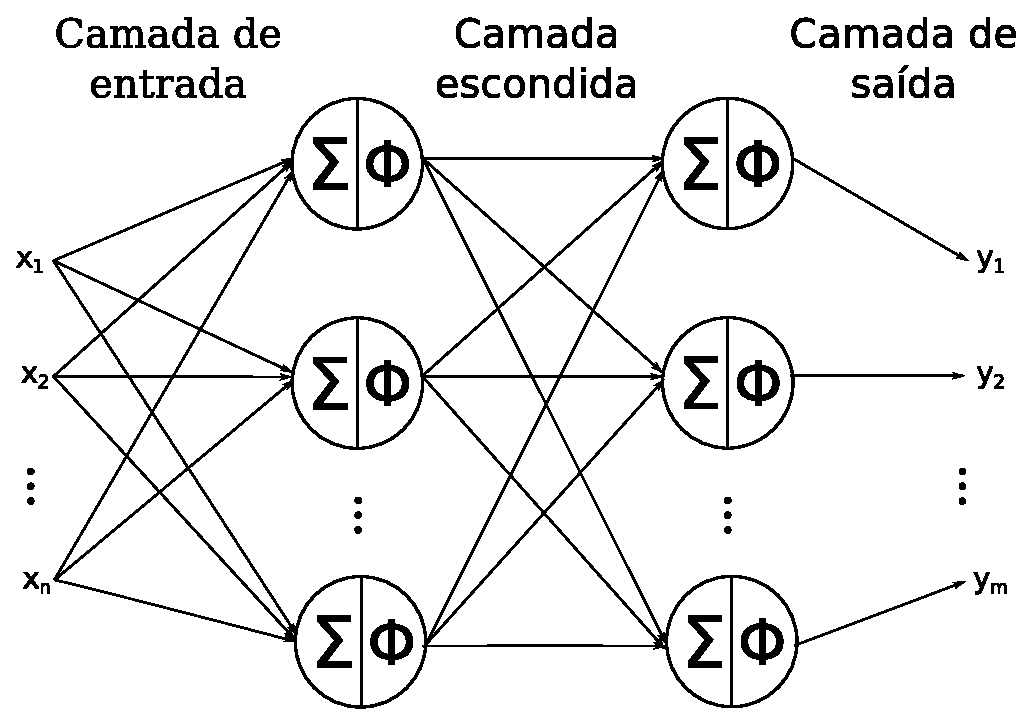
\includegraphics[width=0.4\textwidth]{figures/mlp}
    \caption{Multi-layer Perceptron}
    \label{fig:mlp}
\end{figure}

A saída (y) de um neurônio é determinada pela aplicação de uma função de ativação \(\theta\) sobre a combinação linear ponderada de todas as suas \(n\) entradas \((x_1, x_2, \dots , x_n)\).

Matematicamente,

\[ y = \theta ( \sum_{i=1}^{n} w_i x_i ) \]

onde \(w_i\) é um peso associado a entrada \(i\).

Diversas funções pode assumir o papel de função de ativação, sendo as mais comuns:
a função degrau (\ref{eq:degrau}) e a função sigmóide (\ref{eq:sigmoid}).

\begin{equation} \label{eq:degrau}
    \theta(x) = \left\{
    \begin{array}{l l}
        0 & \quad \text{se } x < 0\\
        1 & \quad \text{caso contrário}
    \end{array} \right.
\end{equation}

\begin{equation} \label{eq:sigmoid}
    \theta(x) = \frac{1}{1 + e^{-x}}
\end{equation}

É comum encontrar, em cada uma das camadas, um neurônio adicional cuja entrada é sempre \(1\). Este neurônio especial tem o nome de \textit{bias} e a finalidade de deslocar a função de ativação para direita ou esquerda.

O ajuste dos pesos \((w_1, w_2, \dots , w_n)\) é chamado treinamento e existe em duas formas:

\begin{description}
    \item[Supervisionado]: É fornecido ao algoritmo de treinamento um conjunto de entradas/saídas. O algoritmo iterativamente ajusta os pesos da rede a fim de que, dadas entradas do conjunto de treinamento, as saídas da rede aproximem-se das saídas.
    \item[Não supervisionado]: Não demanda conjunto de treinamento, os pesos
são ajustados considerando a aptidão da rede à solução do problema.
\end{description}

\subsection{Time-Delay Neural Network (TDNN)}

Estendendo os conceitos das redes MLP, uma TDNN permite à cada neurônio armazenar um
histórico dos sinais de entrada. Isto permite que a rede ganhe sensibilidade à padrões temporais, ou seja, a rede pode adaptar-se não só à padrões como também à sequência de padrões \cite{kaiser94tdnn}.

Este modelo de rede neural é de especial importância na área de robótica. As ações determinadas pelo controlador de um robô devem levar em conta o histórico sensorial e não apenas o estado sensorial atual.

\section{Controle de robôs móveis por RNA}

% ann as robot controller

% [zhang 2000]
% Although many types of neural networks can be used
% for classification purposes [105], our focus nonetheless is on
% the feedforward multilayer networks or multilayer perceptrons
% (MLPs) which are the most widely studied and used neural net-
% work classifiers.

\section{Algoritmos de otimização para treinamento de RNA}
\label{optimization-algorithms}

ga, pso, dpso, bpso, pga